% -*- coding: utf-8 -*-
\section{Introduktion}
Vi ønsker i denne øvelse at implementere en lyd-encoder lignende den som benyttes i MPEG 1 Audio layer 1. Nærmere bestemt ønsker vi at implementere subband-kodning og efterfølgende kvantisering baseret på den menneskelige høretærskel samt spektral maskering.

I figur \ref{blokdiagram} vises et blokdiagram over vores encoders konstruktion.

\begin{figure}[h!]
\begin{center}
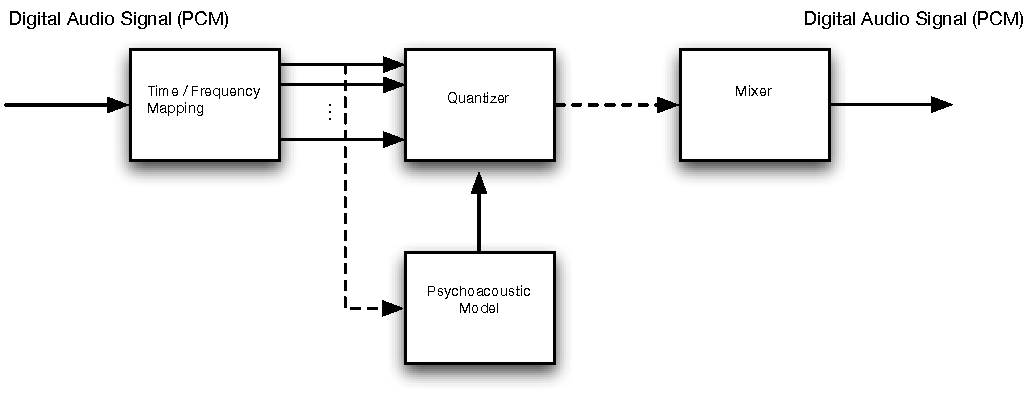
\includegraphics[width=12cm]{blokdiagram}\\
\end{center}
\label{blokdiagram}
\caption{Encoderens konstruktion}
\end{figure}

Der tages ikke højde for MPEG audio-filstandarden; vi ønsker kun at afprøve de tekniske byggeklodser i MPEG audio codec.
